\chapter{Coding / Implementation}

\section{Introduction}
This chapter describes the implementation of \ShortTitle{} including technology choices, directory structure, major classes/modules, API design, and representative algorithms. The complete source code is available in the project repository folder \texttt{canteen-preorder/}.

\section{Technology Stack}
\begin{table}[H]
  \centering
  \caption{Implementation stack}
  \tablebodysetup
  \begin{tabularx}{\textwidth}{@{}l Y@{}}
    \toprule
    \textbf{Layer} & \textbf{Technology} \\
    \midrule
    Frontend & React 19, Next.js 16 App Router, Tailwind CSS 4 \\
    Backend & Next.js API Routes (serverless-ready) \\
    ORM & Prisma 6 \\
    Database & PostgreSQL (Docker locally; cloud for deploy) \\
    Auth & JWT (jose), bcryptjs password hash \\
    QR & qrcode (generate), html5-qrcode + BarcodeDetector (scan) \\
    Charts & Recharts (staff forecast) \\
    Validation & Zod (API request bodies) \\
    \bottomrule
  \end{tabularx}
\end{table}

\section{Directory Structure}
\begin{lstlisting}[caption={Project layout (abbreviated)}]
canteen-preorder/
  prisma/schema.prisma      -- User, MenuItem, Order, OrderItem
  prisma/seed.ts            -- Demo accounts and menu
  src/app/api/              -- REST endpoints
  src/components/           -- StudentApp, StaffApp, UI
  src/components/student/   -- Mobile menu, cart sheet, nav
  src/components/staff/     -- Queue, inventory, forecast
  src/lib/                  -- auth, inventory, qr, fetch-client
  public/manifest.webmanifest
  public/sw.js              -- Service worker (PWA)
  docs/batu-project-report/ -- This LaTeX report
\end{lstlisting}

\section{Database Schema Implementation}
Prisma models implement the E-R design: \texttt{User} (role enum), \texttt{MenuItem} (stock fields), \texttt{Order} (token, status enums), \texttt{OrderItem} (line quantities). Enums \texttt{OrderStatus} and \texttt{PaymentStatus} enforce valid transitions at the application layer.

\section{API Implementation Summary}
Each route validates session role via \texttt{requireSession}. Table~\ref{tab:api} lists endpoints.

\begin{table}[H]
  \centering
  \caption{API endpoints}
  \label{tab:api}
  \tablebodysetup
  \begin{tabularx}{\textwidth}{@{}l l Y@{}}
    \toprule
    \textbf{HTTP} & \textbf{Path} & \textbf{Description} \\
    \midrule
    POST & /api/auth & Login / register \\
    GET & /api/auth/session & Current user \\
    GET & /api/menu & Menu + daily special + stock labels \\
    POST & /api/cart/validate & Stock validation for cart \\
    POST & /api/orders & Create PENDING order \\
    GET & /api/orders & Student order history \\
    POST & /api/payments & Pay; deduct stock; CONFIRMED \\
    GET & /api/orders/[id]/qr & QR data URL \\
    GET & /api/orders/queue & Staff queue \\
    POST & /api/orders/verify & Verify token/QR \\
    POST & /api/orders/[id]/confirm-handover & COMPLETED \\
    PATCH & /api/inventory & Stock / availability update \\
    GET & /api/forecast & Demand forecast JSON \\
    \bottomrule
  \end{tabularx}
\end{table}

\section{Module Descriptions}

\subsection{Authentication (\texttt{src/lib/auth.ts})}
\textbf{Purpose:} Issue and verify JWT stored in HTTP-only cookie \texttt{session}.

\textbf{Methods:}
\begin{itemize}
  \item \texttt{createSession(user)} --- Input: user record; Output: Set-Cookie header.
  \item \texttt{getSession()} --- Input: request cookies; Output: payload or null.
  \item \texttt{requireSession(roles[])} --- Input: allowed roles; Output: user or 401/403.
\end{itemize}

\subsection{Inventory (\texttt{src/lib/inventory.ts})}
\textbf{Purpose:} Business rules for stock display and mutation.

\textbf{Methods:}
\begin{itemize}
  \item \texttt{getStockStatus(qty, threshold)} $\rightarrow$ \texttt{available|low|out}.
  \item \texttt{enrichMenuItem(row)} $\rightarrow$ adds \texttt{canOrder}, \texttt{availabilityLabel}.
  \item \texttt{validateCartItems(lines)} $\rightarrow$ array of errors or valid flag.
  \item \texttt{deductStockForOrder(orderId)} $\rightarrow$ transactional decrement per line.
\end{itemize}

\subsection{Student Application (\texttt{StudentApp.tsx})}
\textbf{Purpose:} Single-page student workflow with steps \texttt{menu}, \texttt{review}, \texttt{payment}, \texttt{receipt}.

\textbf{Key state variables:} \texttt{cart}, \texttt{step}, \texttt{pendingOrder}, \texttt{paidOrder}, \texttt{mobileTab}.

\textbf{Features:} Category filter, bottom cart bar, mobile cart sheet, checkout step bar (compact on mobile), active order banner, visibility-aware polling (\texttt{useVisibilityPolling}), toast on add-to-cart.

\subsection{Staff Application (\texttt{StaffApp.tsx})}
\textbf{Purpose:} Tabbed staff UI: queue, verify (QR scanner), inventory, forecast.

\textbf{Inventory PATCH body:}
\begin{lstlisting}[caption={Custom stock update examples}]
{ "menuItemId": "...", "stockQuantity": 17 }  // set exact count
{ "menuItemId": "...", "addStock": 30 }       // add to current
{ "menuItemId": "...", "isAvailable": false } // sold out online
\end{lstlisting}

\subsection{QR Library (\texttt{src/lib/qr.ts})}
Encodes order ID and verification fields in QR payload. \texttt{parseQrPayload} and \texttt{verifyPayloadBody} normalize scanner output for \texttt{/api/orders/verify}.

\subsection{Forecast (\texttt{src/lib/forecast.ts})}
Aggregates completed orders over 14 days, computes weighted moving average per menu item, outputs \texttt{suggestedPrep} and trend indicator (up/down/stable).

\section{User Interface Components}
The main React components used in the student and staff interfaces are listed in Table~\ref{tab:ui-components}.

\begin{table}[H]
  \centering
  \caption{Major UI components}
  \label{tab:ui-components}
  \tablebodysetup
  \begin{tabularx}{\textwidth}{@{}l Y@{}}
    \toprule
    \textbf{Component} & \textbf{Role} \\
    \midrule
    MenuItemRow & Compact menu line with +/- controls \\
    BottomCartBar / MobileCartSheet & Mobile checkout entry \\
    OrderReceipt / FullscreenQrModal & Token + QR display \\
    StaffTabBar & Horizontal staff navigation \\
    InventoryStockControls & Add / Set to / +10 / +25 \\
    PwaInstallPanel & Install instructions per platform \\
    NetworkStatusBanner & Offline user feedback \\
    \bottomrule
  \end{tabularx}
\end{table}

\section{Algorithms}

\subsection{Stock Validation (Cart)}
For each cart line, fetch menu item; if \texttt{!isAvailable} or \texttt{quantity > stockQuantity}, append error with message; return HTTP 409 if any error.

\subsection{Payment and Stock Deduction}
On successful payment API: verify order PENDING; re-validate stock; update order to PAID/CONFIRMED; assign token; call \texttt{deductStockForOrder}; return order JSON for receipt view.

\subsection{Token Generation}
Unique \texttt{tokenNumber} (e.g.\ A154) and \texttt{orderCode} (e.g.\ ORD-2026-54) generated at payment time with collision checks against database unique constraints.

\section{Screenshots of the Developed System}
\label{sec:ui-screenshots}
Figures~\ref{fig:login}--\ref{fig:staff-verify} show the main screens of \ShortTitle{} captured from the running application on a mobile viewport.

% UI screenshots — include from chapter06-coding.tex
% Requires images/*.png and \hasimagestrue in student-info.tex

\ifhasimages

\begin{figure}[htbp]
  \centering
  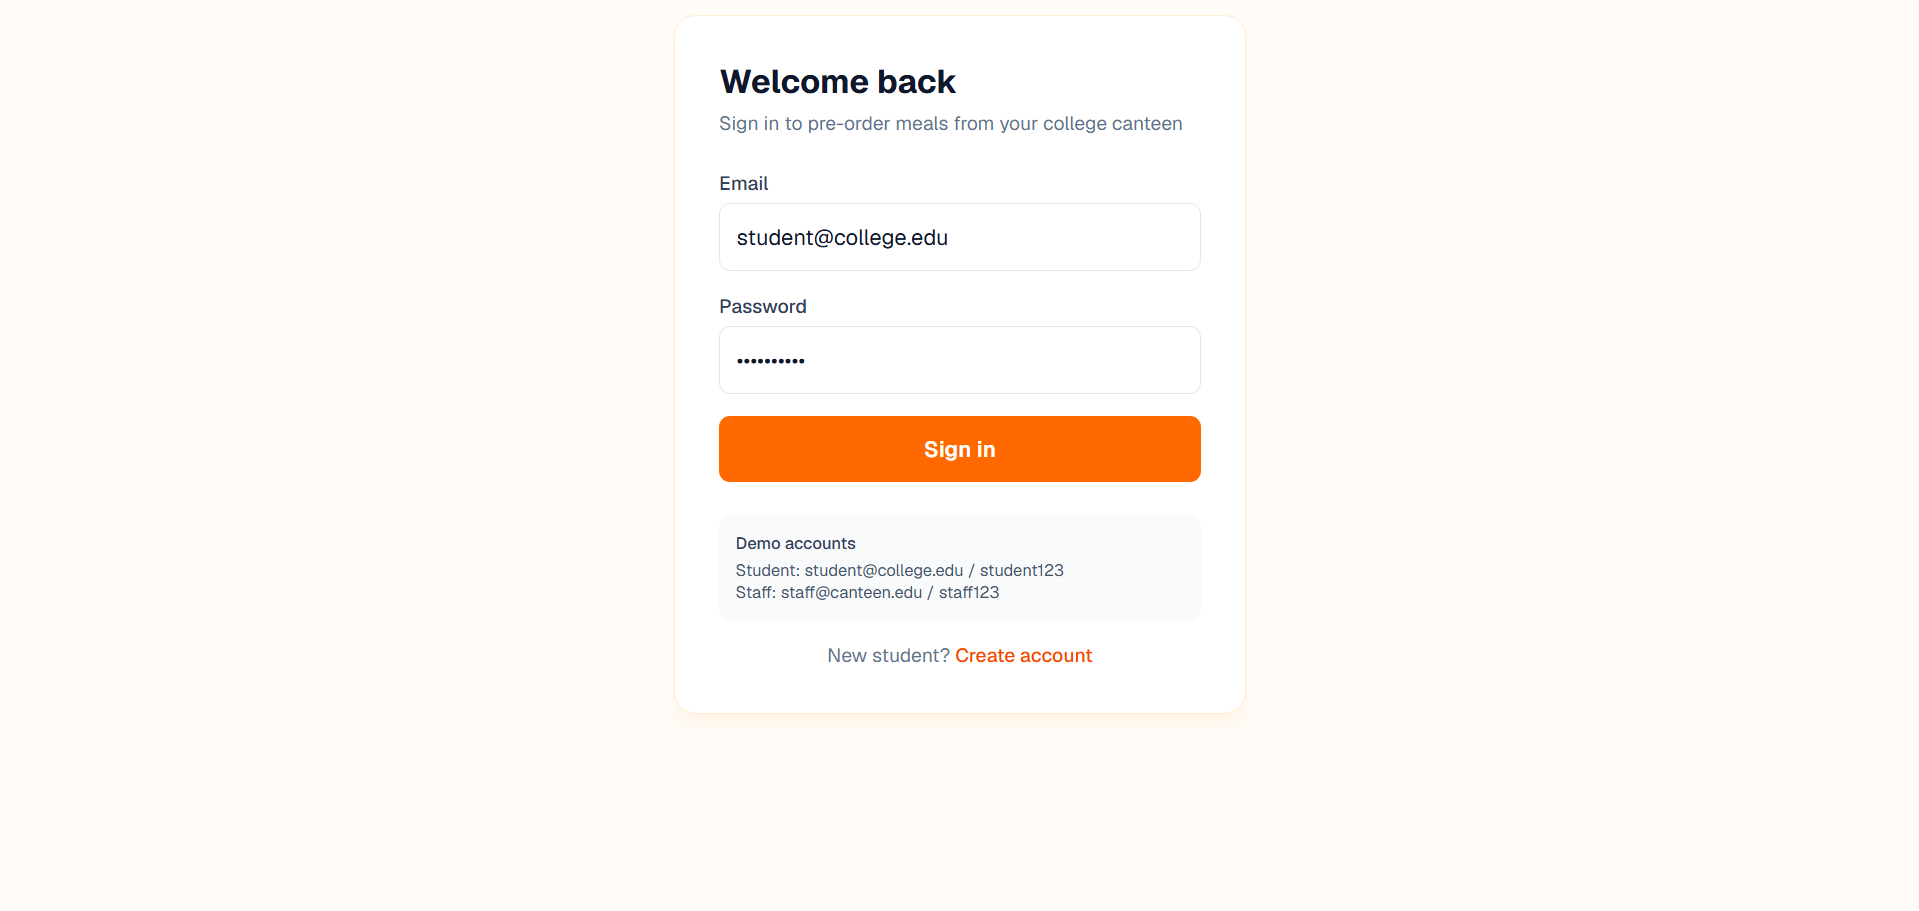
\includegraphics[width=0.85\textwidth]{images/01-login.png}
  \caption{Login page --- student and staff credentials}
  \label{fig:login}
\end{figure}

\begin{figure}[htbp]
  \centering
  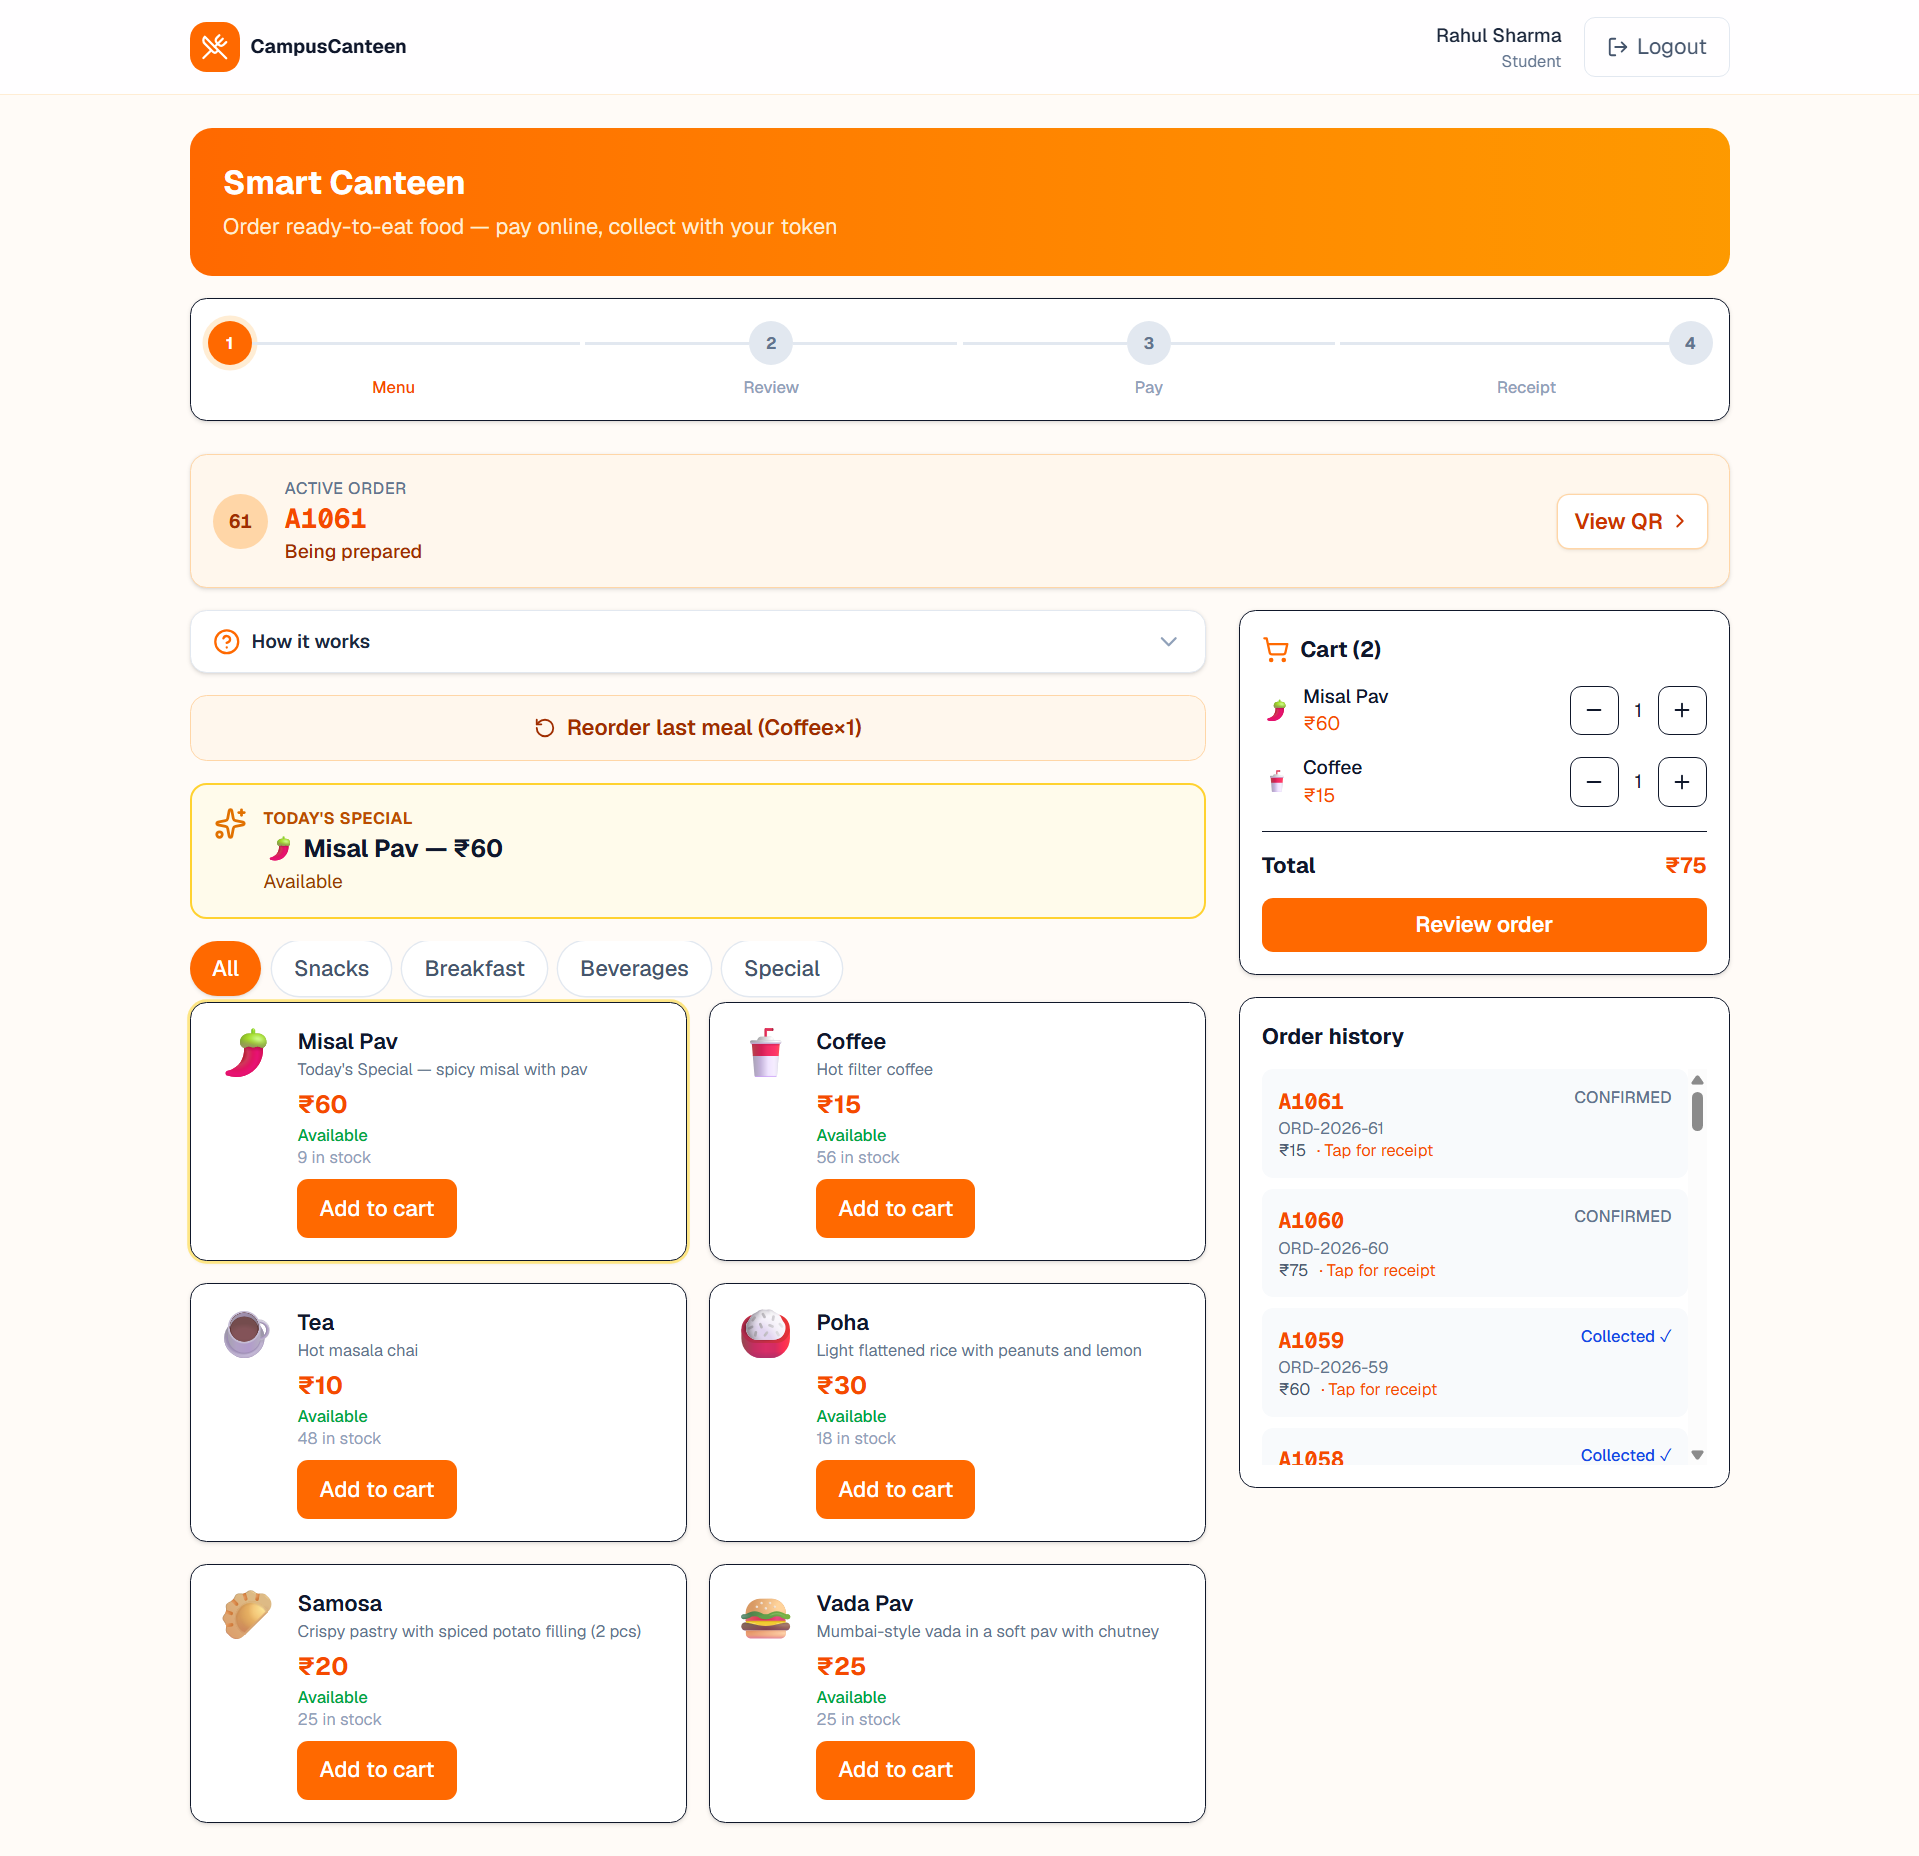
\includegraphics[width=0.85\textwidth]{images/02-student-menu.png}
  \caption{Student menu screen (mobile layout) with categories and stock labels}
  \label{fig:student-menu}
\end{figure}

\begin{figure}[htbp]
  \centering
  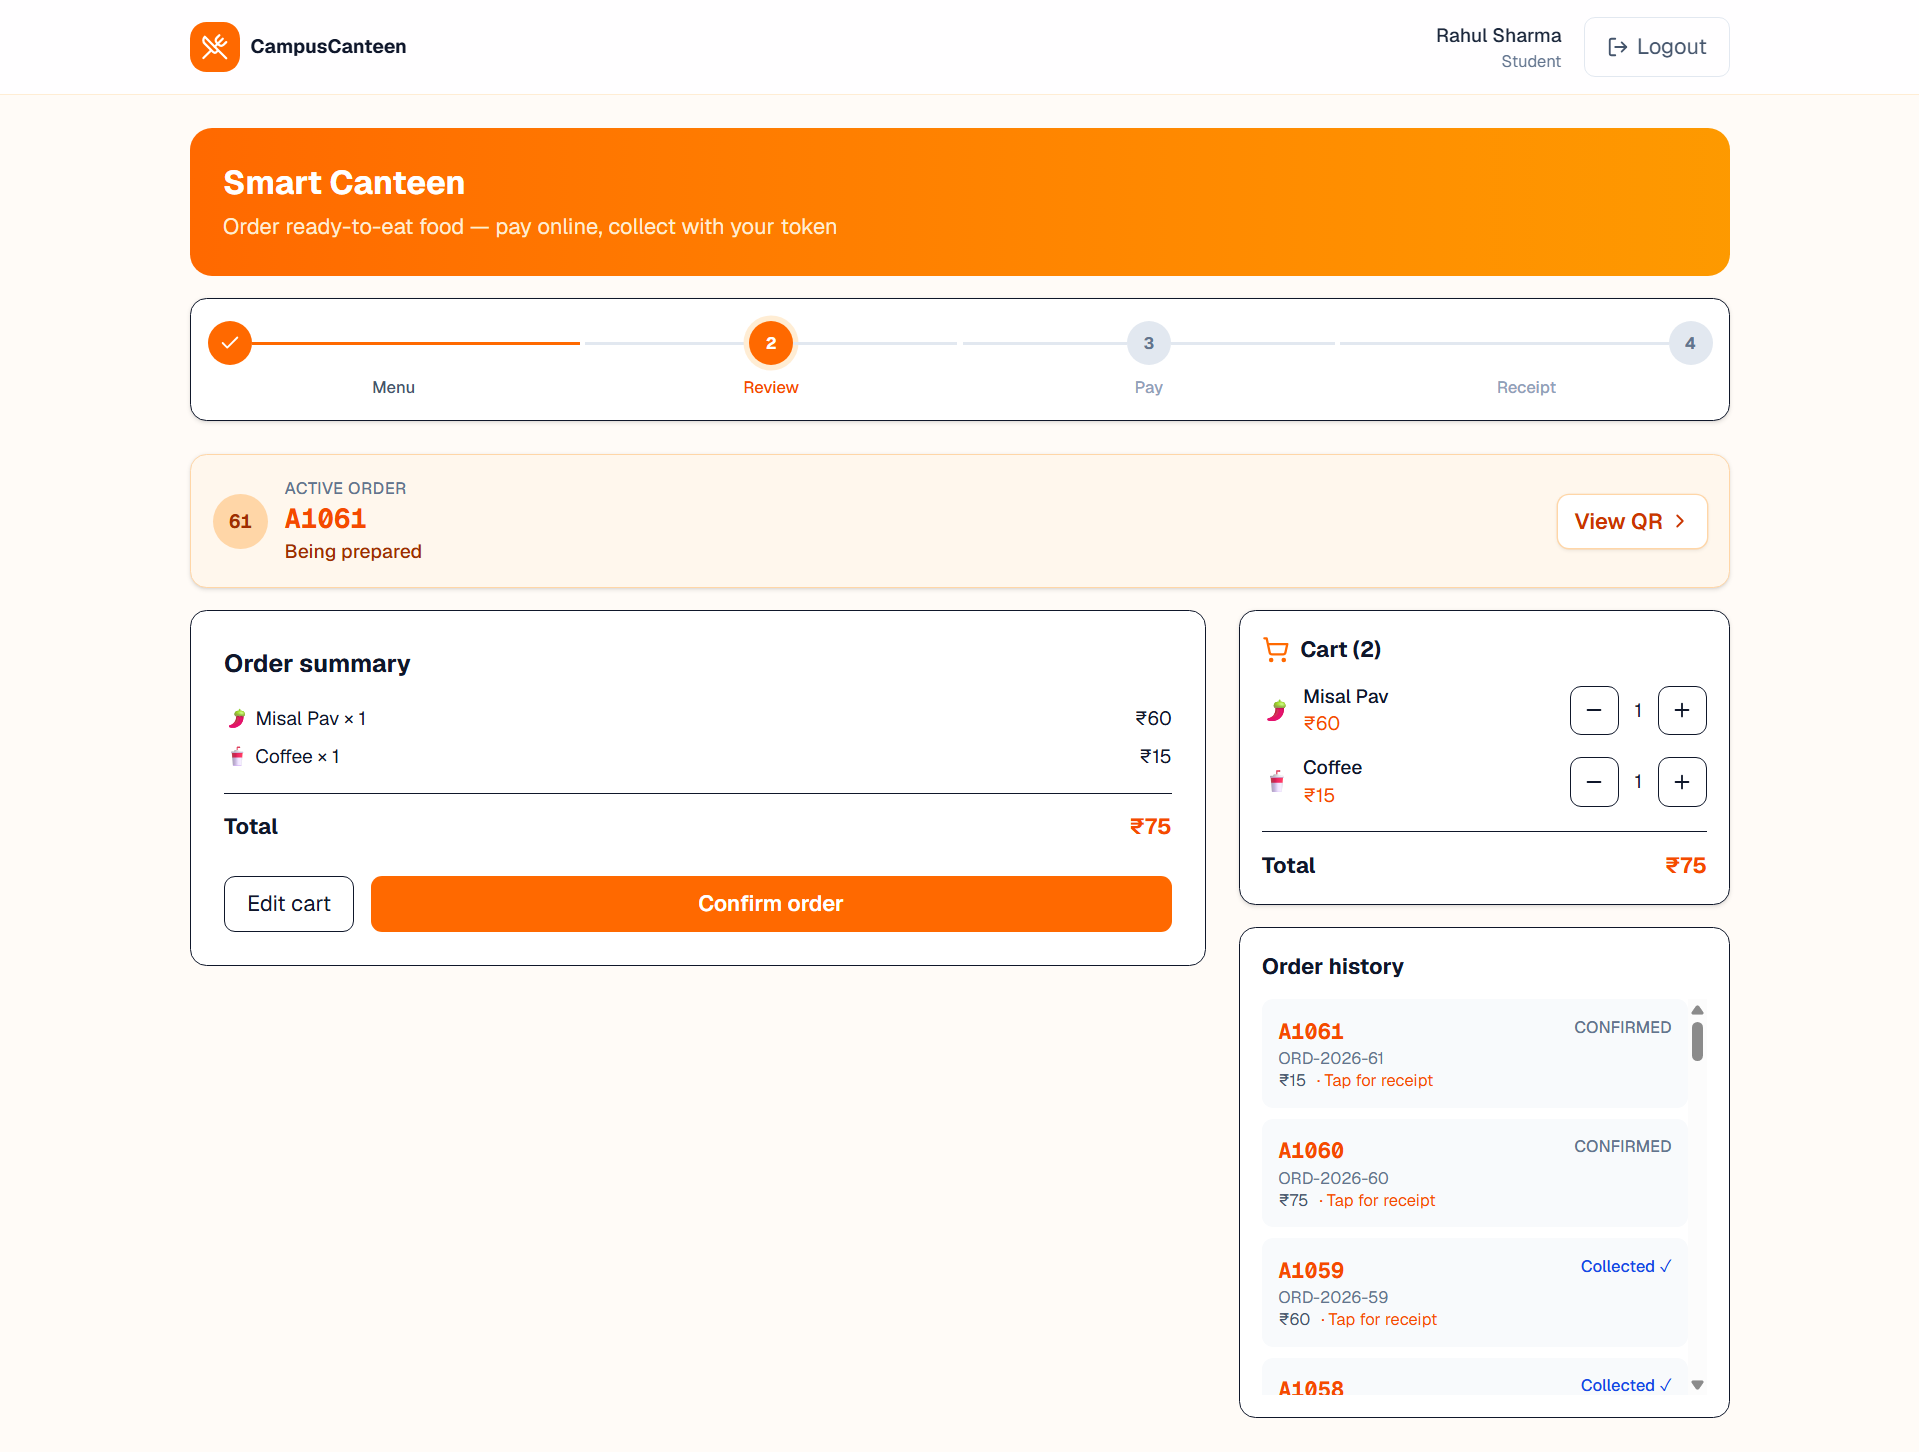
\includegraphics[width=0.85\textwidth]{images/03-review-order.png}
  \caption{Order review step before payment}
  \label{fig:review-order}
\end{figure}

\begin{figure}[htbp]
  \centering
  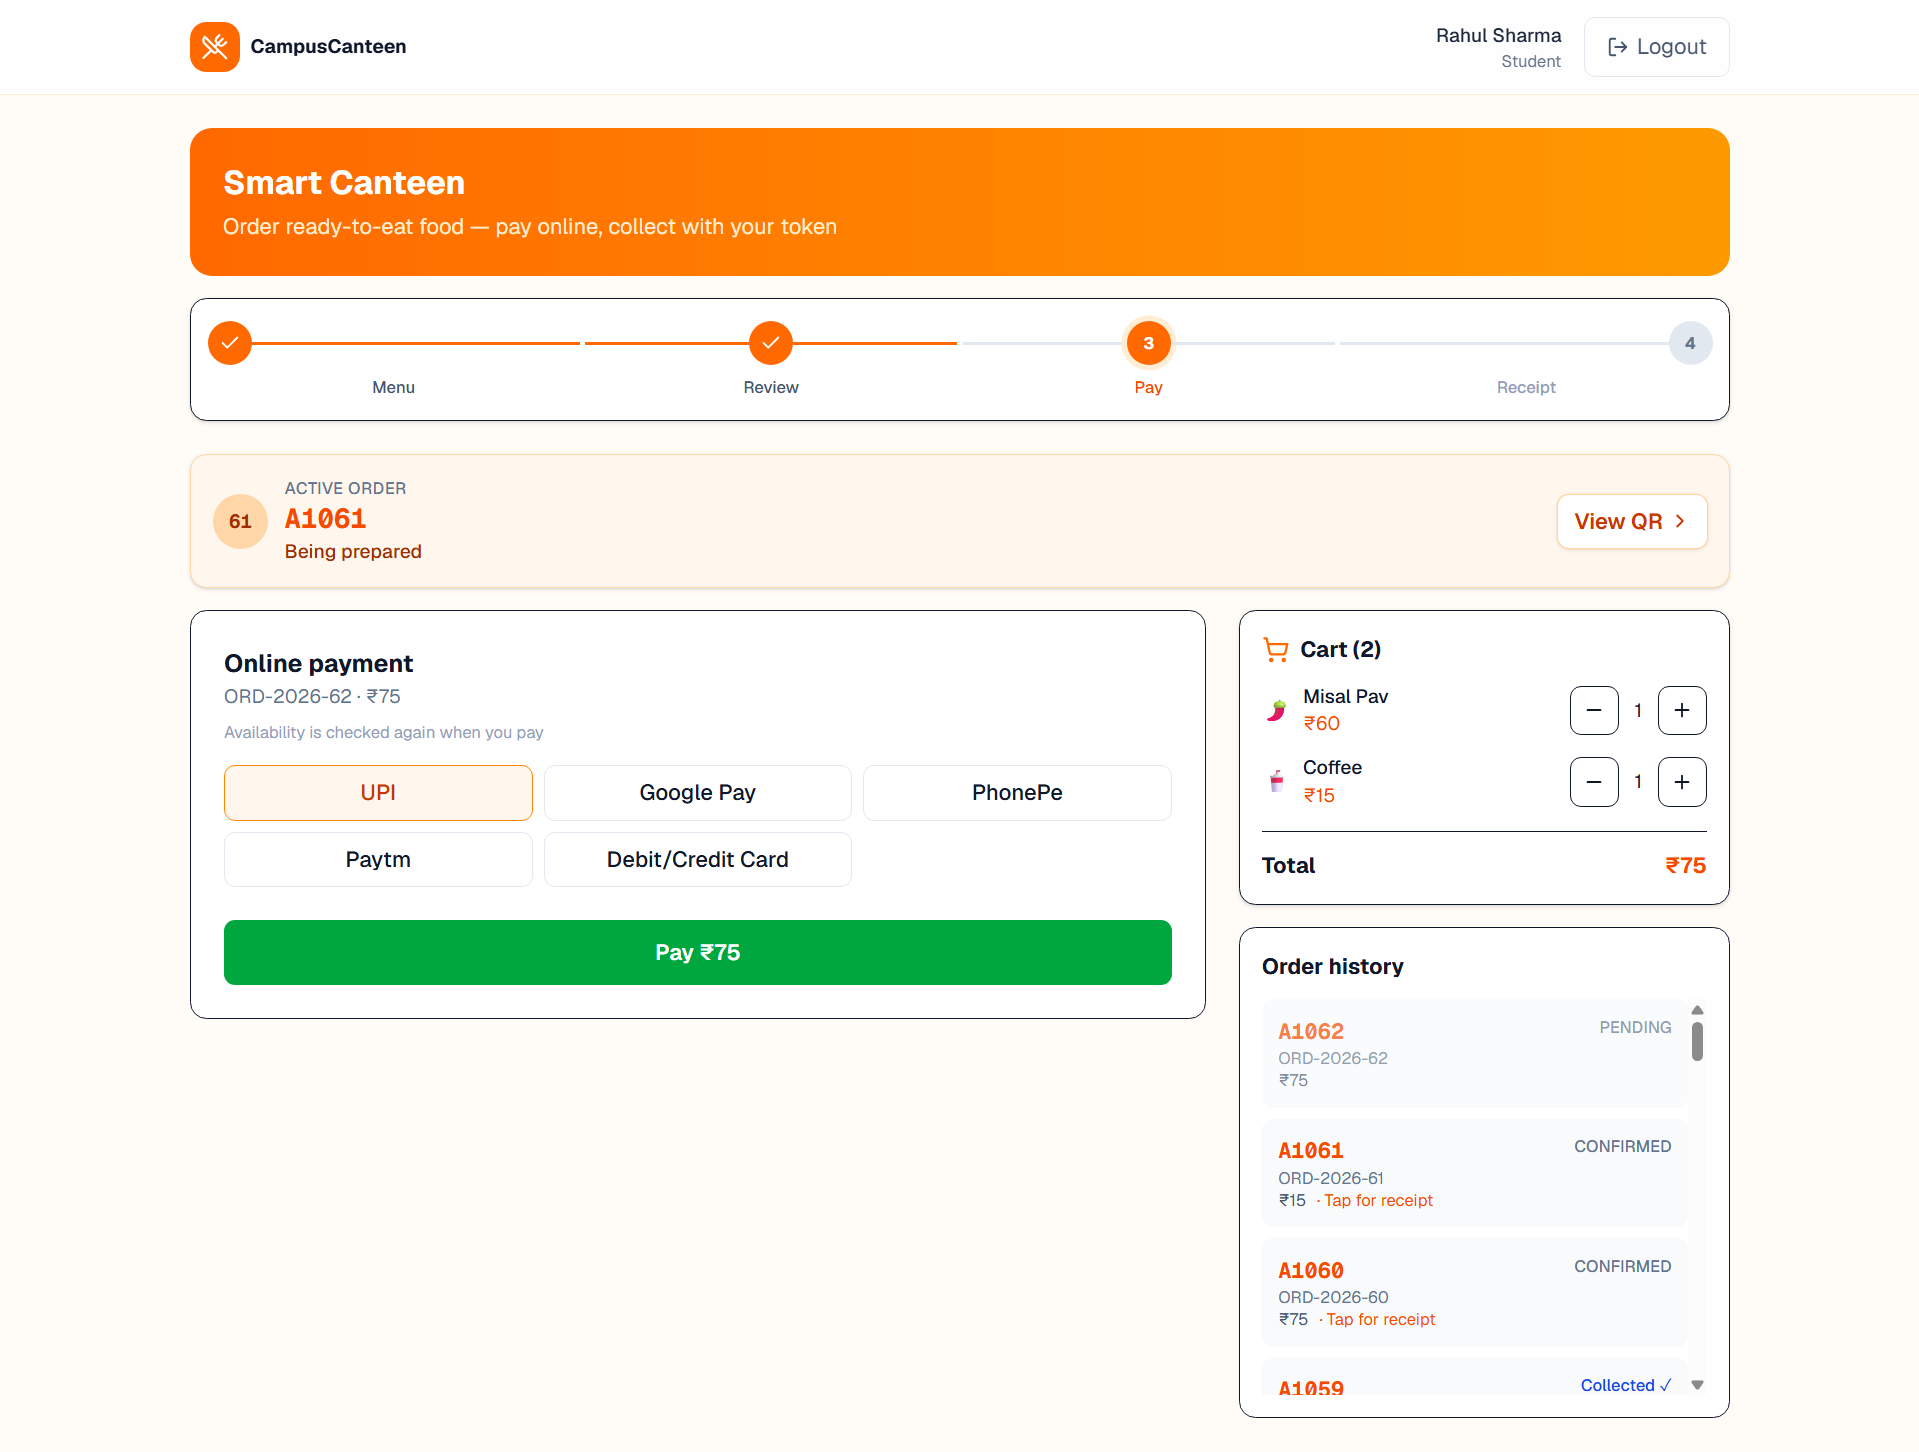
\includegraphics[width=0.85\textwidth]{images/04-payment.png}
  \caption{Payment confirmation screen}
  \label{fig:payment}
\end{figure}

\begin{figure}[htbp]
  \centering
  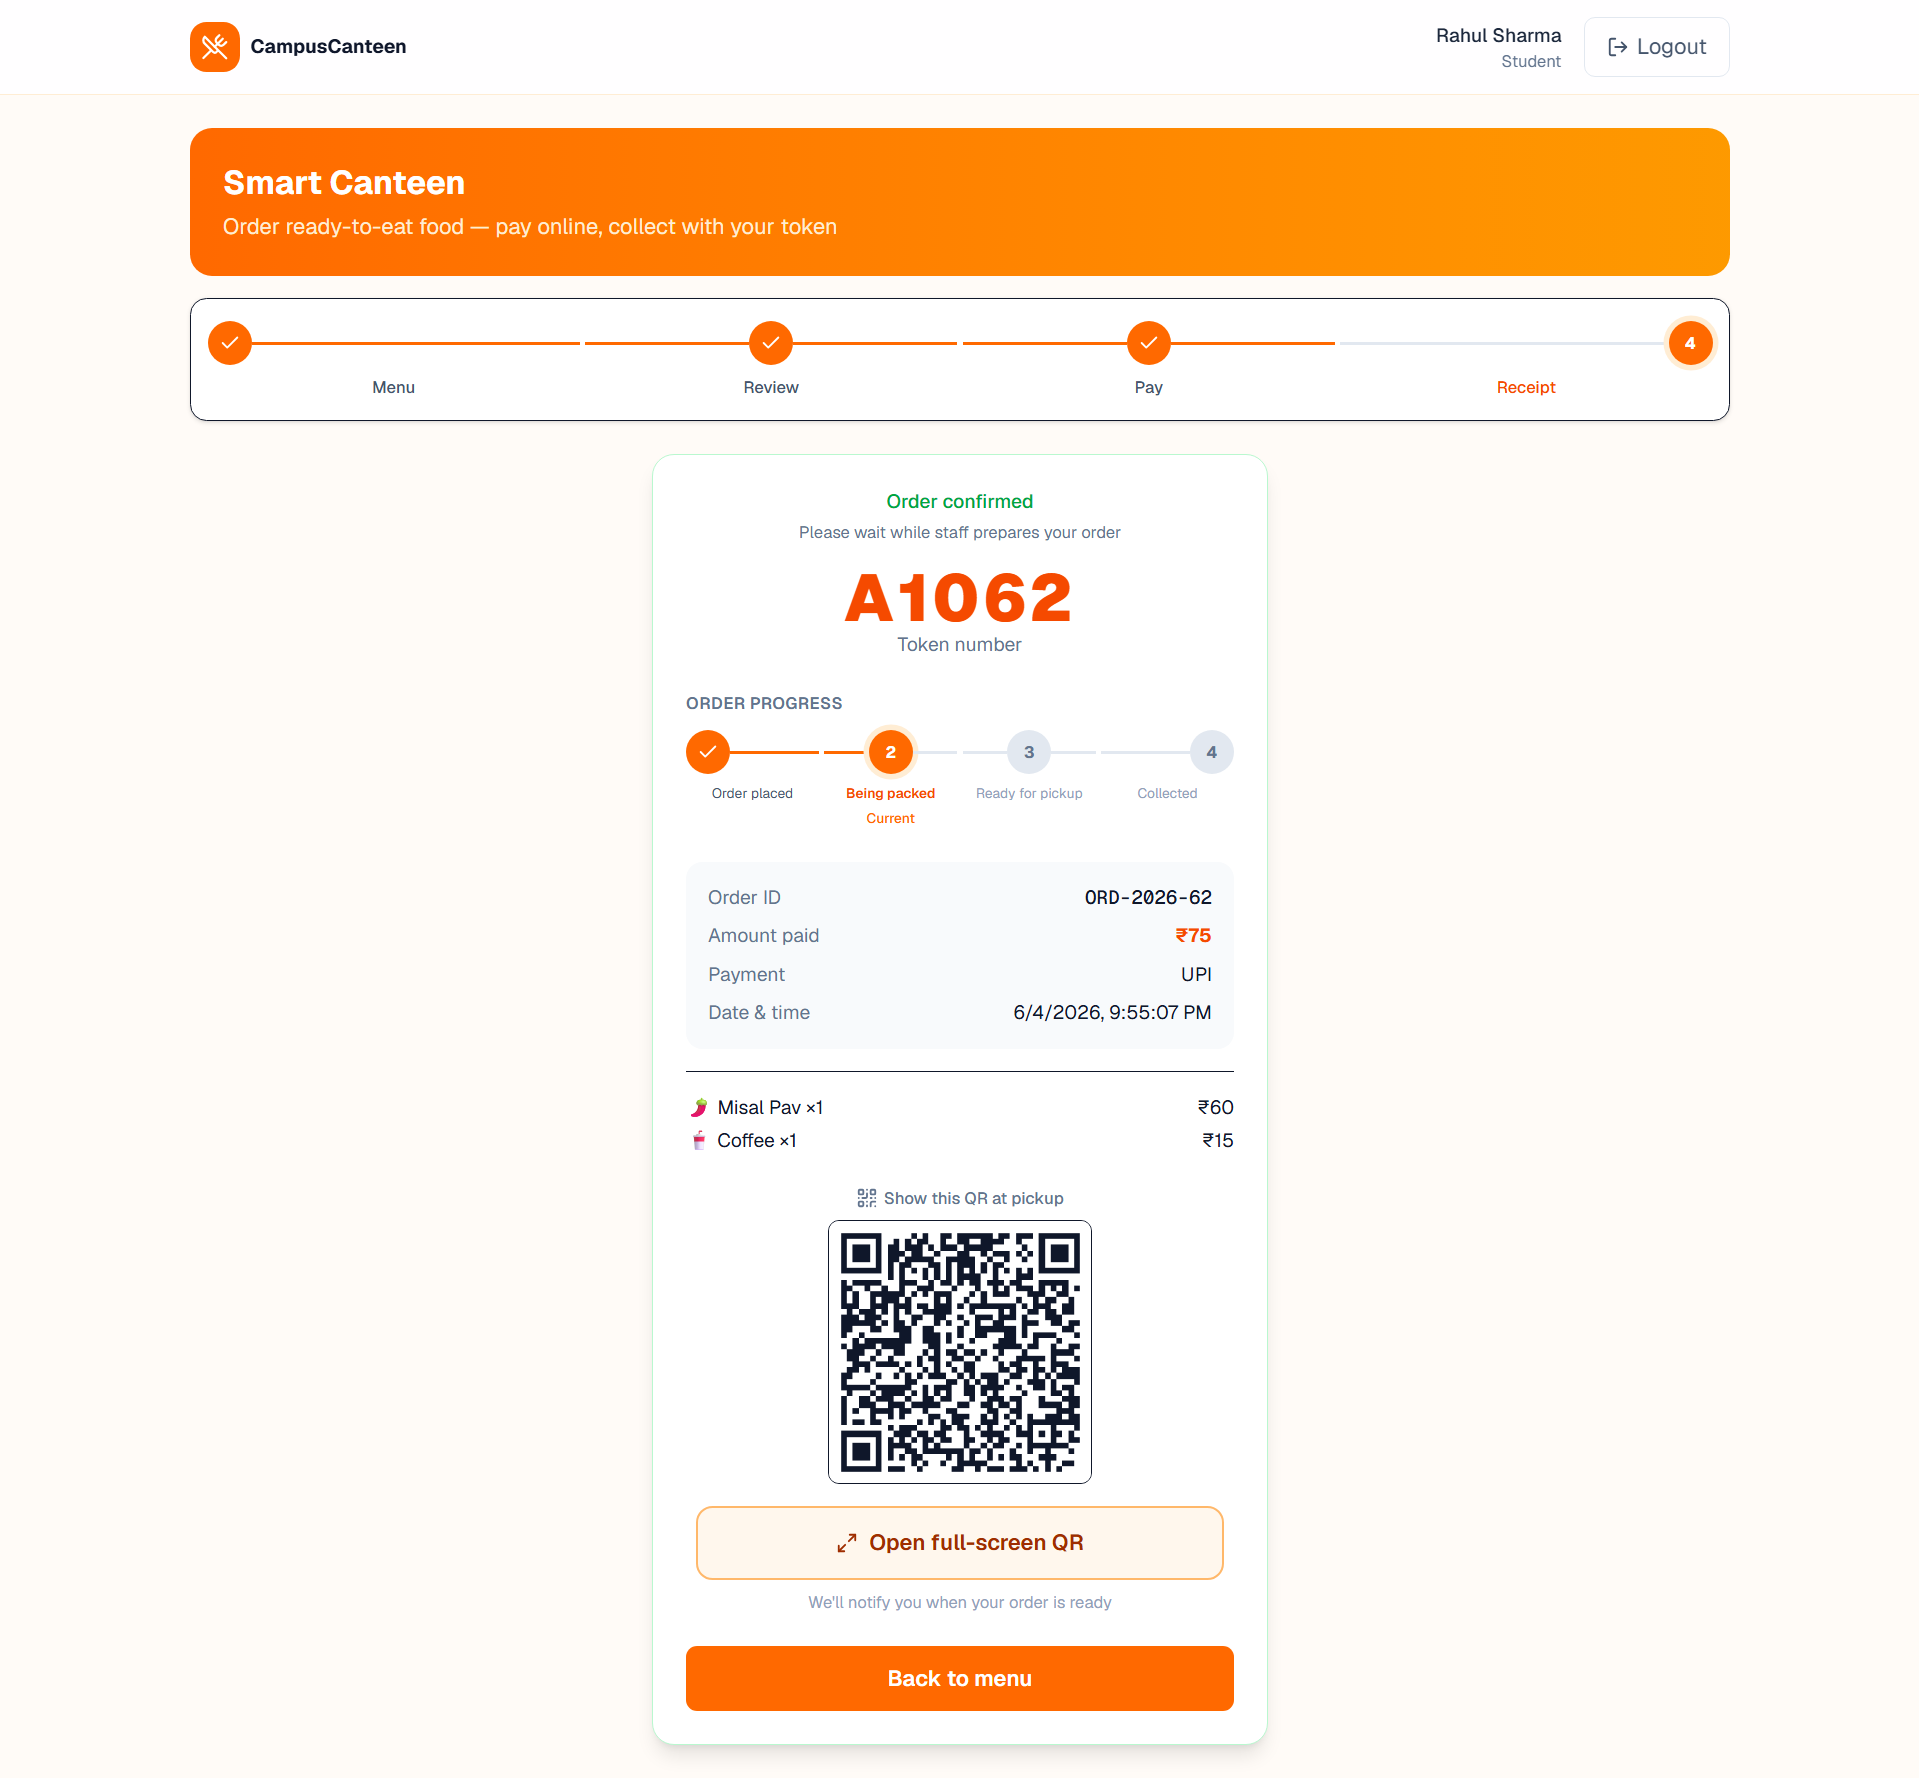
\includegraphics[width=0.85\textwidth]{images/05-receipt-qr.png}
  \caption{Order receipt with pickup token and QR code}
  \label{fig:receipt-qr}
\end{figure}

\begin{figure}[htbp]
  \centering
  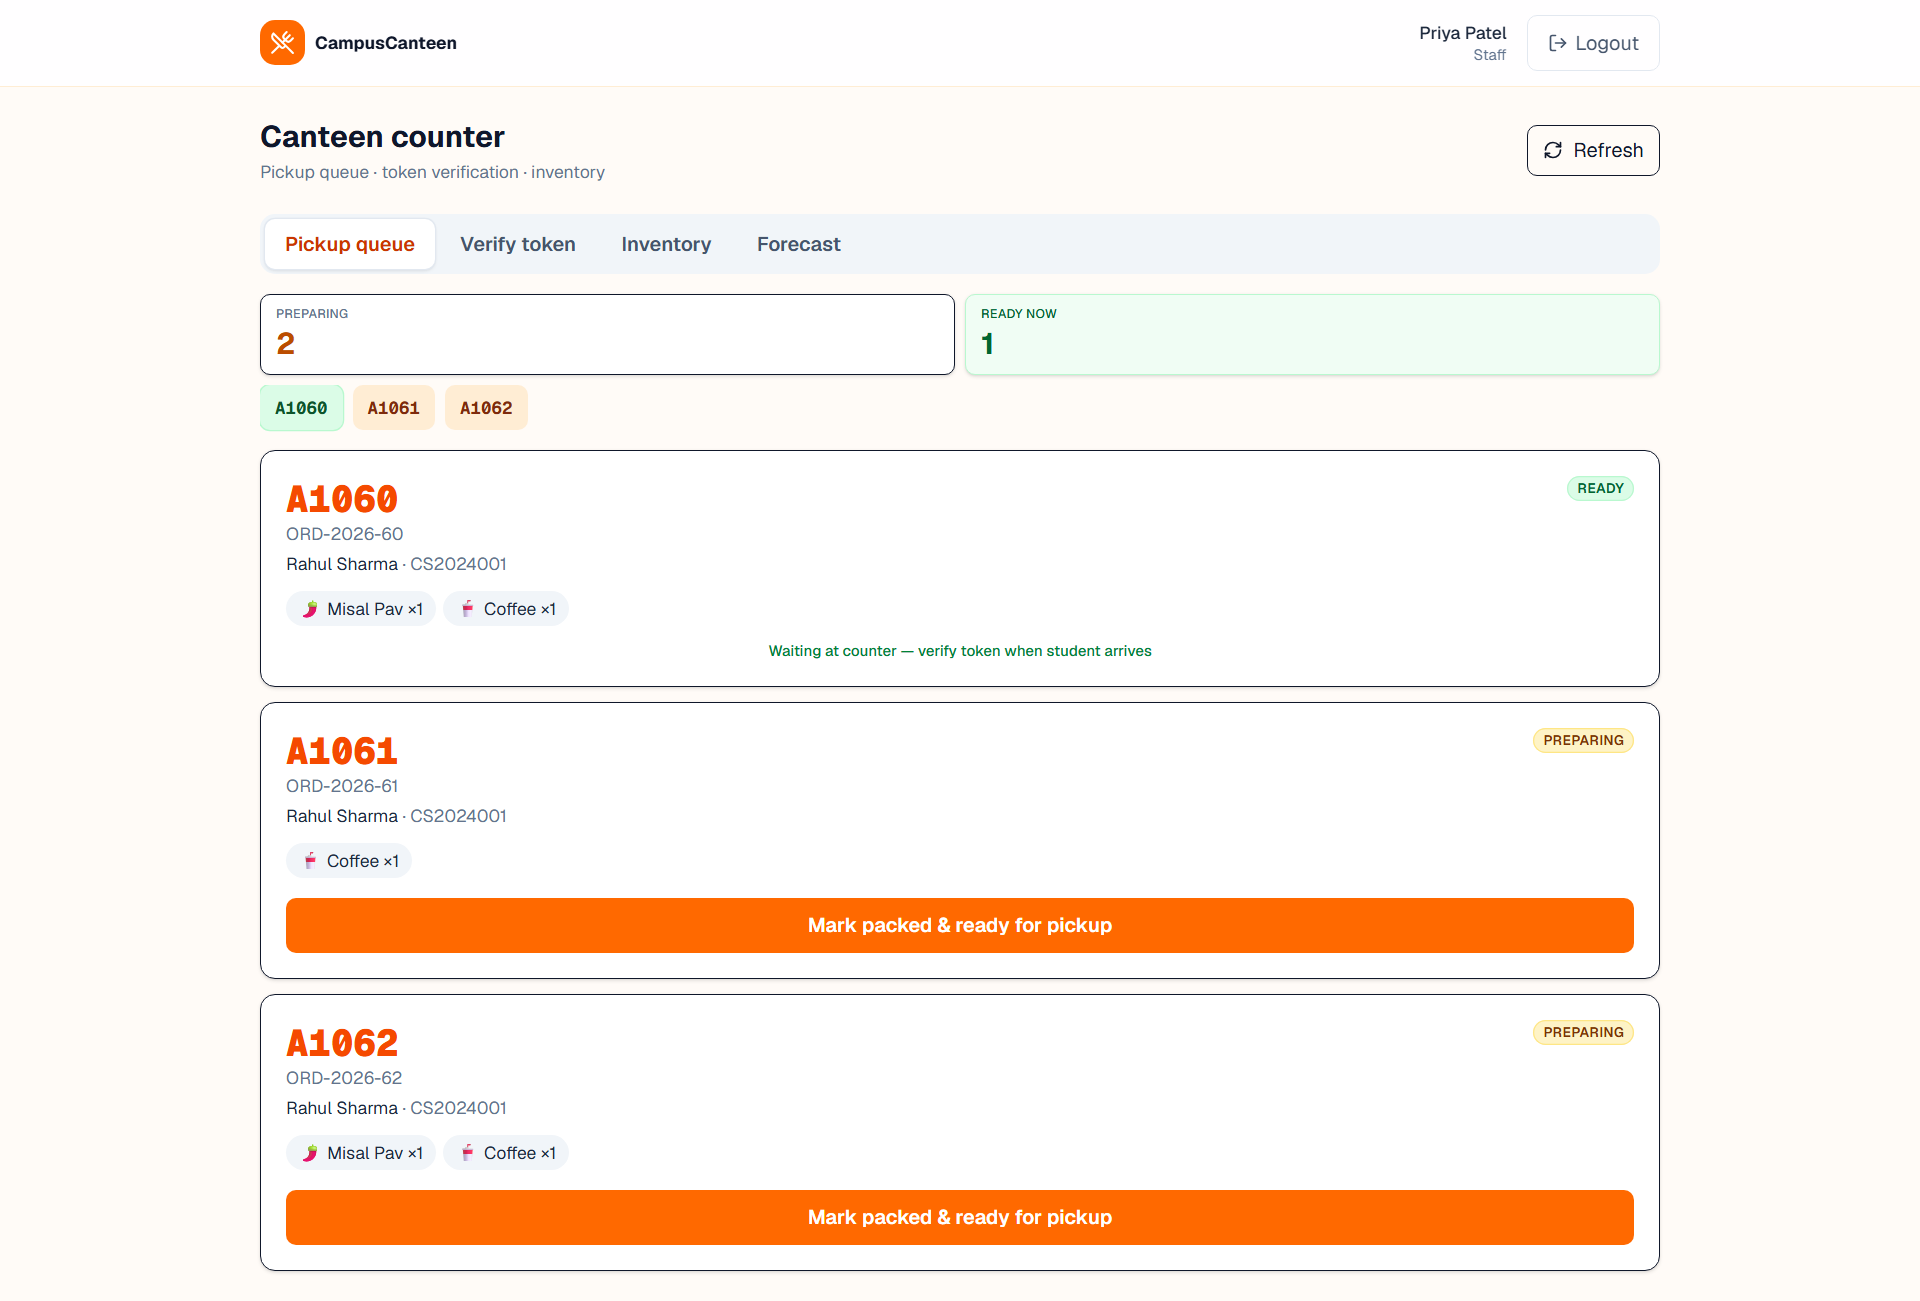
\includegraphics[width=0.85\textwidth]{images/06-student-orders.png}
  \caption{Student ``My orders'' tab with order status}
  \label{fig:student-orders}
\end{figure}

\begin{figure}[htbp]
  \centering
  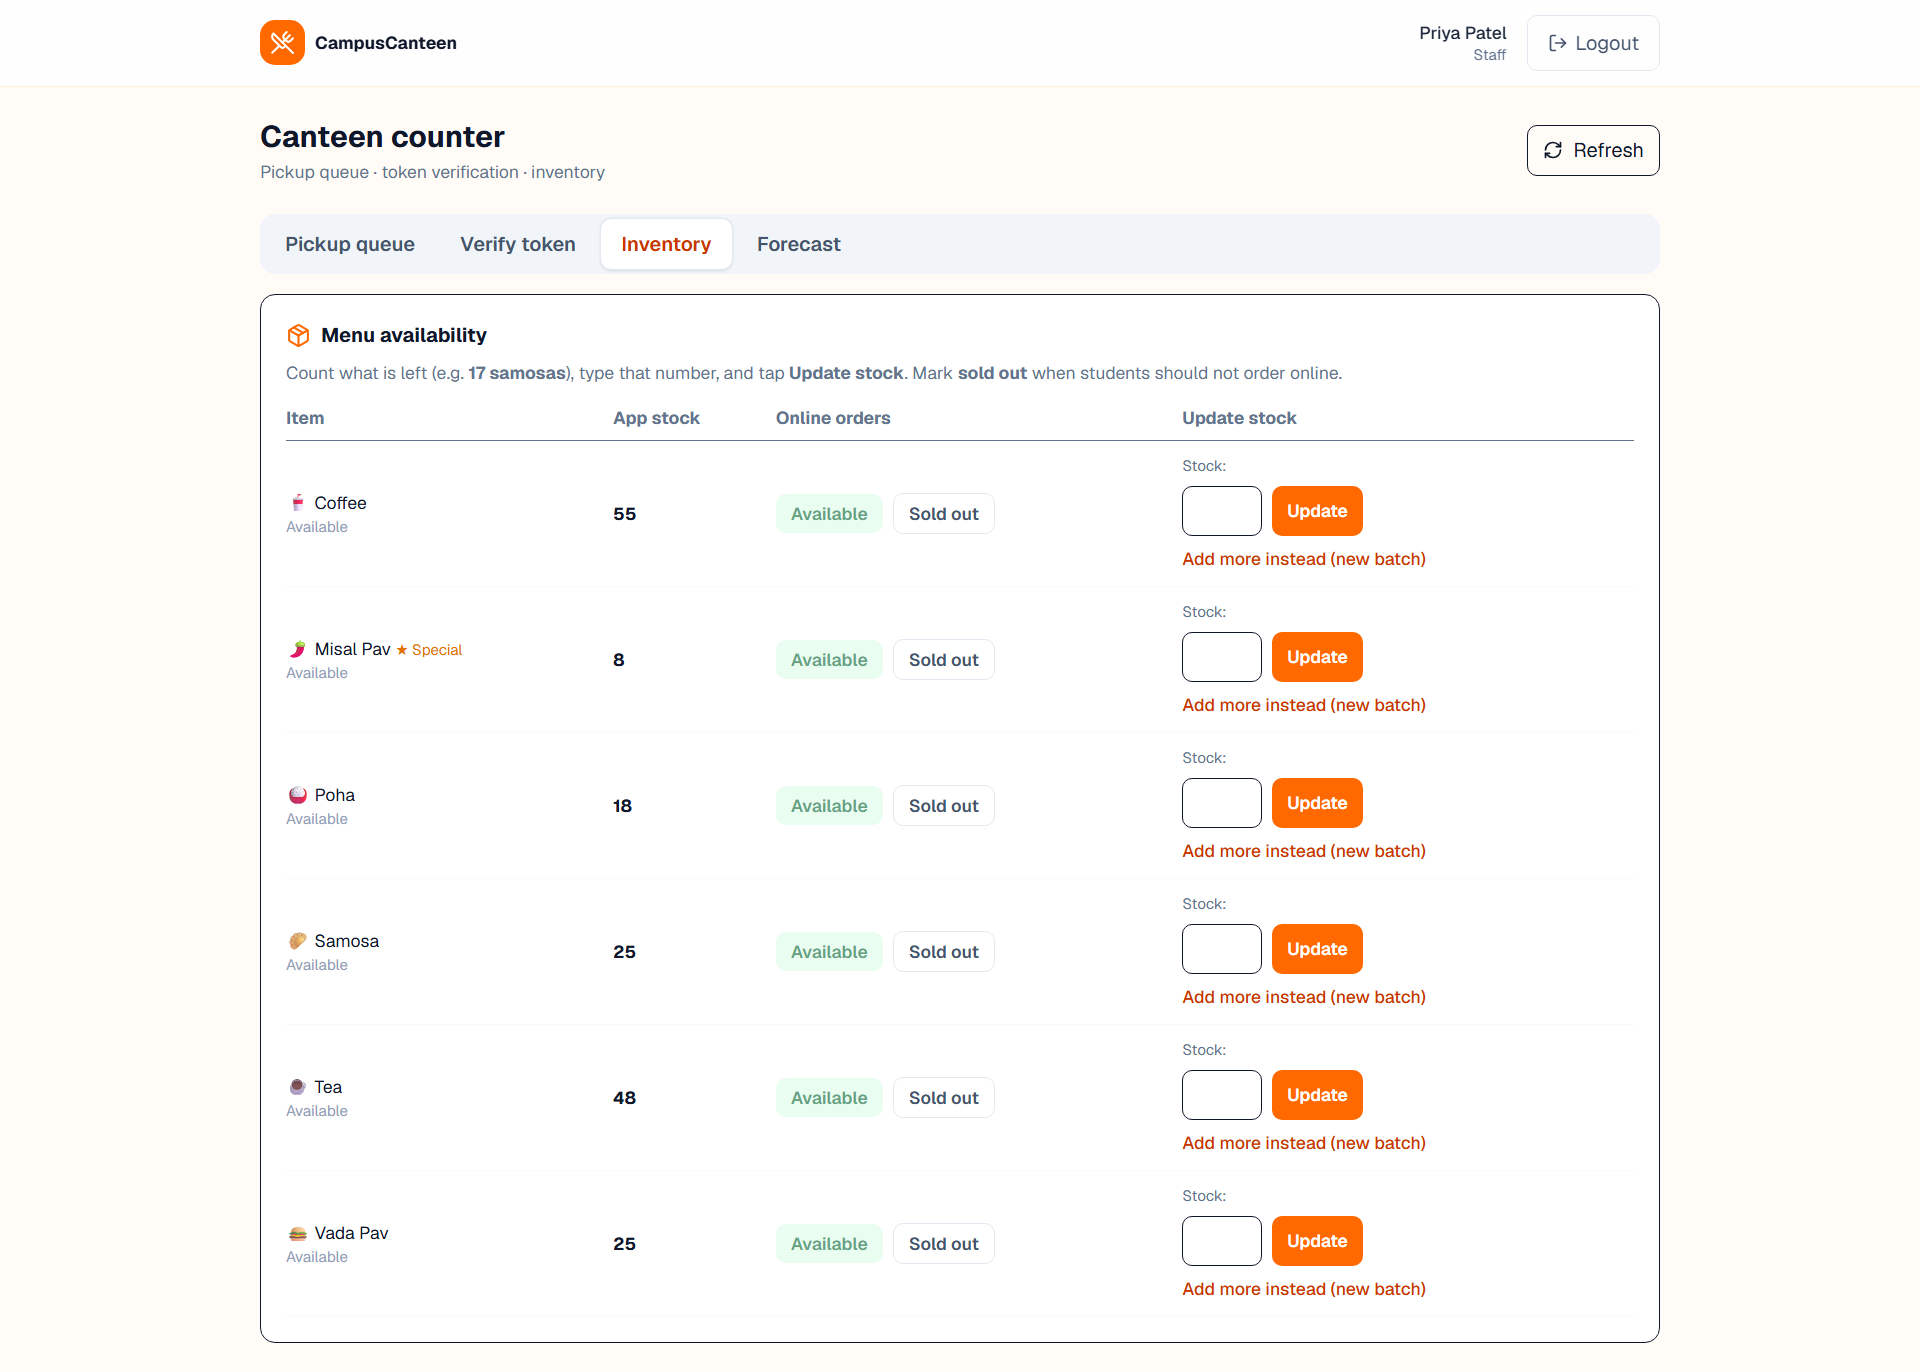
\includegraphics[width=0.85\textwidth]{images/07-staff-inventory.png}
  \caption{Staff inventory management with custom ``Set to'' stock (e.g.\ 17 samosas)}
  \label{fig:staff-inventory}
\end{figure}

\begin{figure}[htbp]
  \centering
  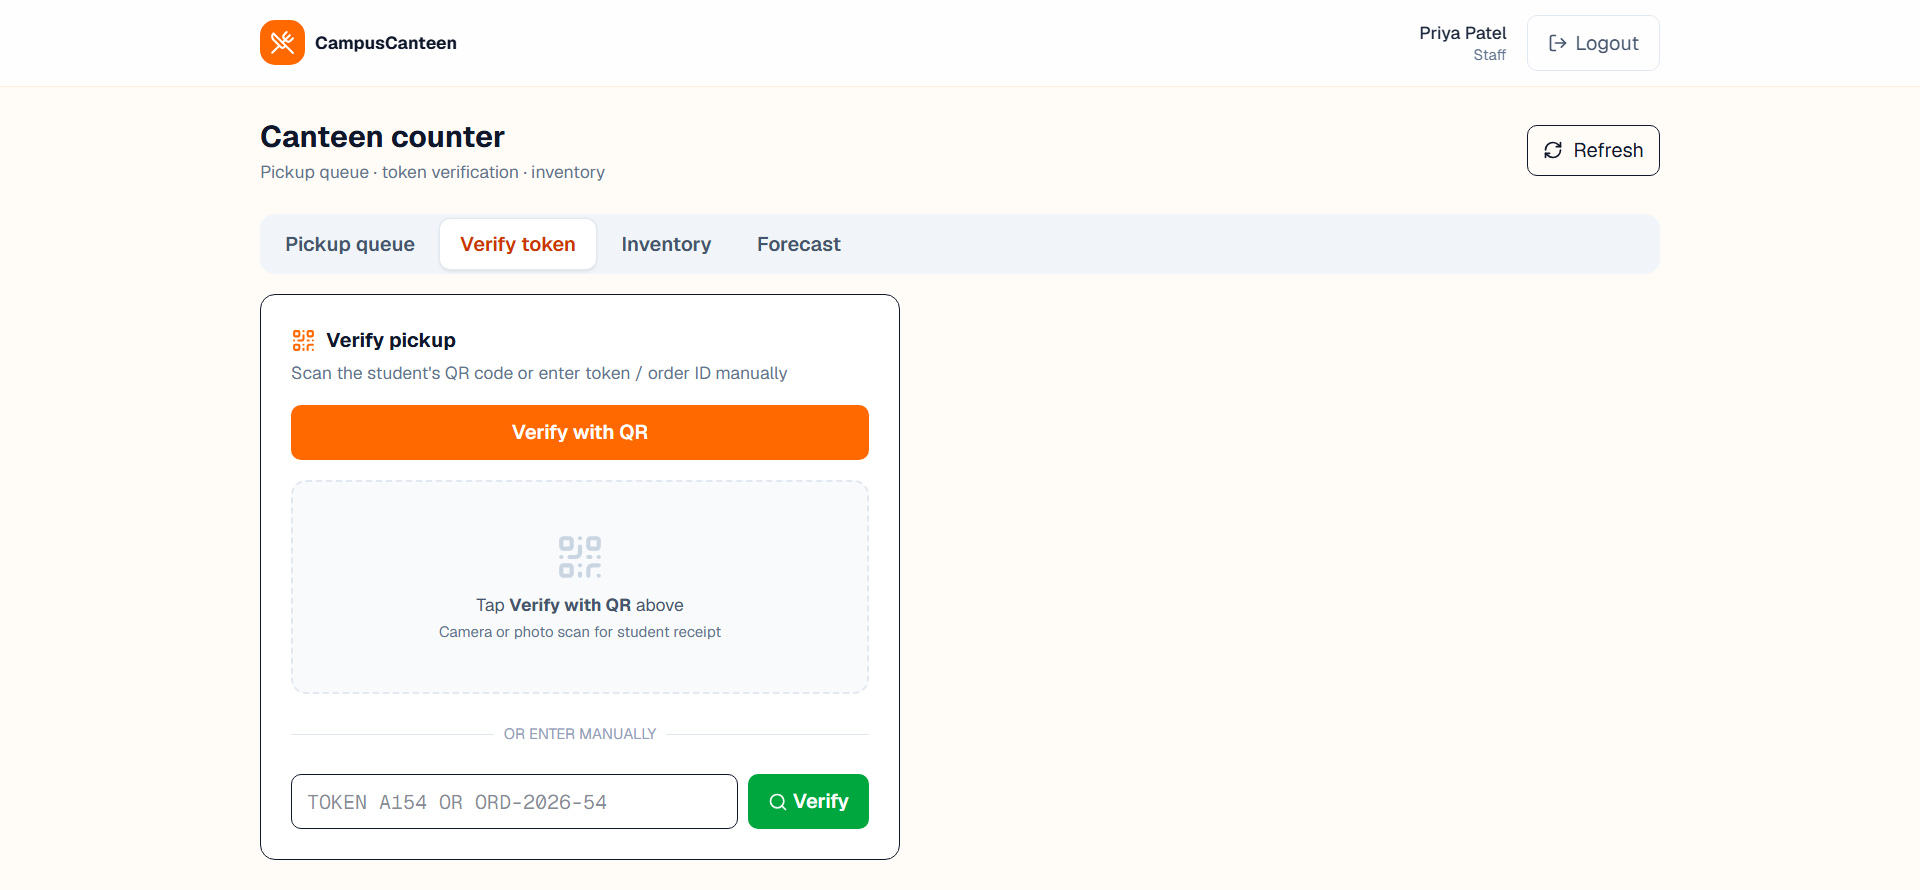
\includegraphics[width=0.85\textwidth]{images/08-staff-verify.png}
  \caption{Staff QR verification and handover screen}
  \label{fig:staff-verify}
\end{figure}

\else

\noindent\textcolor{red}{\textbf{[Screenshots not included yet.]}}
Add PNG files listed in Table~\ref{tab:screenshot-checklist} to the folder \texttt{images/}, then set \texttt{\textbackslash hasimagestrue} in \texttt{student-info.tex} and recompile twice so the List of Figures updates.

\fi


\section{Testing Approach}
Manual test cases are documented in Appendix~\ref{app:tests}. Testing included mobile viewport in Chrome DevTools, LAN access from Android phone, staff QR scan, and inventory update to arbitrary stock value.

\section{Version Control}
Project developed with Git. Recommended practice: commit after each milestone (auth, student flow, staff flow, mobile UI, inventory PATCH).
